\newcommand\chapternumber{3}
\documentclass[12pt,a4paper]{article}
\usepackage{fullpage}
\usepackage[top=2cm, bottom=4.5cm, left=2.5cm, right=2.5cm]{geometry}
\usepackage{amsmath,amsthm,amsfonts,amssymb,amscd}
\usepackage{lastpage}
% \usepackage{enumitem}
\usepackage{fancyhdr}
\usepackage{mathrsfs}
\usepackage{xcolor}
\usepackage{graphicx}
\usepackage{listings}
\usepackage{hyperref}
\usepackage{tikz}
\usetikzlibrary{shapes,backgrounds}
\usepackage[utf8]{inputenc}
\usepackage[ruled, vlined]{algorithm2e}
% \usepackage{apacite}
\usepackage{csquotes}

% Edit these as appropriate
\newcommand\course{Data Science II}
\newcommand\NetID{sliu1@uvm.edu}
\newcommand\Author{Sida Liu}
\pagestyle{fancyplain}
\headheight 35pt
\lhead{\NetID\\\Author}
\chead{\textbf{\Large \pagetitle }}
\rhead{\course \\ \today}
\lfoot{}
\cfoot{}
\rfoot{\small\thepage}
\headsep 1.5em

\setlength{\parskip}{\baselineskip}%
\setlength{\parindent}{0pt}%

\newenvironment{list_abc}
{ \begin{enumerate}[label=(\alph*)] }
    { \end{enumerate} }

\newenvironment{list_iv}
{ \begin{enumerate}[label=\roman*.] }
    { \end{enumerate} }

\hypersetup{
  colorlinks=true,
  linkcolor=blue,
  filecolor=magenta,
  urlcolor=cyan,
}

\usepackage[overload]{empheq}
\usepackage{tikz}
\usetikzlibrary{bayesnet}
\usetikzlibrary{arrows}

\usepackage{xparse}
\NewDocumentCommand\Cycle{O{} m m m O{} m}{%
% [opt arg cycle]{Node}{Angle}{Node size}[opt arg arch node]{cycle size}
\draw[#1](#2.{#3+asin(#6/(#4*1.41))}) arc (180+#3-45:180+#3-45-270:#6/2) #5;
}

% no color for hyperlinks
\usepackage{hyperref}
\hypersetup{
  colorlinks=true, 
  citecolor=blue, 
  linkcolor=blue, 
  urlcolor=blue
}

\usepackage{enumerate}
\usepackage{float}

\begin{document}

\section{Manual Gradient Descent}
\begin{align*}
    \frac{\partial \ell_i}{\partial \theta_j} = -2 x_{ij} (y_i - \sum_{j'=1}^{p} x_{ij'} \theta_{j'})\\
\end{align*}
\begin{align*}
    \nabla_{\theta} \ell &= \sum_{i=1}^{N} \begin{bmatrix}
        \frac{\partial \ell_i}{\partial \theta_1} \\
        \frac{\partial \ell_i}{\partial \theta_2} \\
        \vdots \\
        \frac{\partial \ell_i}{\partial \theta_p} \\
    \end{bmatrix}\\\\
    &= -2 x^T (y-x\theta)
\end{align*}

I used the dataset this \href{https://www.kaggle.com/sulianova/cardiovascular-disease-dataset}{Cardiovascular Disease dataset}.

The are 70k records in this dataset.
The task is to predict whether a person has cardiovascular disease or not base on his age, height, etc.
I split the dataset into 80\% training and 20\% testing.

The source code is on \href{https://github.com/liusida/ds2/blob/main/assignment3/code/q1.py}{GitHub}.

I discovered that larger batch size and larger learning rate will result in faster convergence, 
however, if learning rate is too large, the learning might diverge,
and if batch size and learning rate is too large will cause overflow.
So I normalized the input to reduce the possibility of overflow, and choose a batch size of 7k, and a small learning rate.
Now the learning process with 1k epochs takes 1.5 seconds. (If I use a batch size of 100, it will take 9.8 seconds.)

The final test accuracy is 0.643.
I also report the final confusion matrix:
Sensitivity 0.574, Specificity 0.712,
Precision 0.667, Negative Predictive Value 0.625.

Why would I choose to manually do gradient descent?
Because I want to learn how it works, and also, as David mentioned in class, sometimes we have constraints in practice, for example there's possibility that PyTorch is not supported.

\newpage
\section{2D Rosenbrock function}
\begin{figure}[h]
    \includegraphics[width=.99\textwidth]{./rosenbrock.pdf}
    \caption{Visualization of 2D Rosenbrock function. $x \in (-30,30)$, $y \in (-300,800)$}
\end{figure}

It is hard for SGD because the low area is not a dot but a long belt.
If the learning rate is large, it will diverge.
If the learning rate is low, it will be very slow in finding the minima on that flat belt.

Analytically, we need to solve the equations: $\frac{\partial f}{\partial x} = 0$ and $\frac{\partial f}{\partial y} = 0$.

% \[
%     \systeme*{\frac{\partial f}{\partial x} = 0, \frac{\partial f}{\partial y} = 0}
% \]
\begin{align*}[left = \empheqlbrace]
    \frac{\partial}{\partial x} (1-x)^2+100(y-x^2)^2 &= 0\\
    \frac{\partial}{\partial y} (1-x)^2+100(y-x^2)^2 &= 0\\
\end{align*}

\begin{align*}[left = \empheqlbrace]
    400x^3-400xy+2x-2 &= 0\\
    y&=x^2\\
\end{align*}

\begin{align*}
    400x^3-400x^3+2x-2 &= 0\\
    x&=1\\
    y&=1\\
\end{align*}

Using routine gradient descent, start from $x_0=0, y_0=0$, learning rate $\gamma=10^{-3}$, run for 10k steps.
The optimization successfully converged to the minimum.

This is because the initialization is quite close to the minimum,
and because it is smooth in $x \in (0,1)$ and $ y \in (0,1)$.
Figure \ref{fig:routine_gd} shows the trajectory of the optimization.

\begin{figure}[h]
    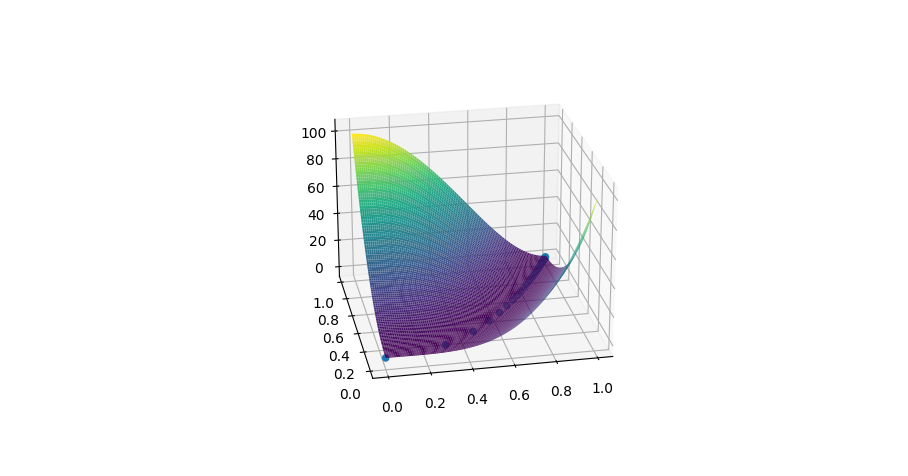
\includegraphics[width=.8\textwidth]{./routine_gd.png}
    \caption{Visualization of the optimization trajectory. $x \in (0,1)$, $y \in (0,1)$.}
    \label{fig:routine_gd}
\end{figure}

If we are not that lucky and use a bad initialization, such as $x_0 = 3$, $y_0 = -2$,
then the routine gradient descent will be harder.
The learning rate need to be smaller, otherwise it will diverge.
Then momentum is needed to speed the optimization up.
I set momentum to 0.99, learning rate $\gamma=10^{-5}$, and run for 10k steps.
The optimization successfully converged to the minimum.
Figure \ref{fig:gd_m} shows the trajectory.

\begin{figure}[h]
    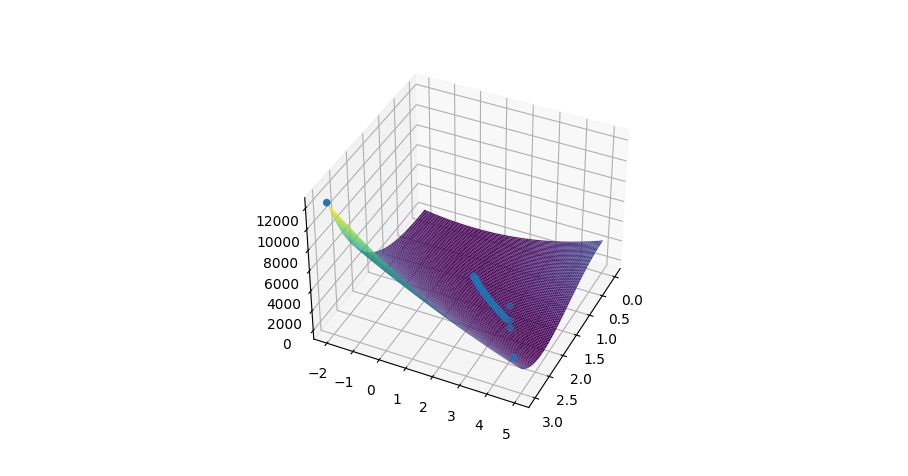
\includegraphics[width=.8\textwidth]{./gd_m.png}
    \caption{Visualization of the optimization trajectory with momentum. $x \in (0,3)$, $y \in (-2,5)$.}
    \label{fig:gd_m}
\end{figure}

\section{}

\end{document}
